\section{Background and Motivation}
\label{sec:background}

\subsection{LLM Architecture and Parallel Stategy}
\label{sec:llmandtransformer}

% \begin{figure}
% 	\centering
% 	\begin{minipage}[t]{\linewidth}
% 		\centering
% 		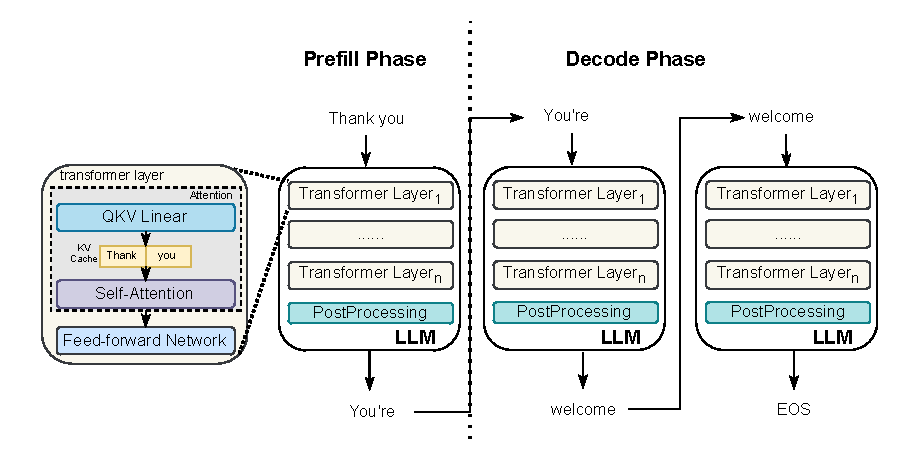
\includegraphics[width=3.3in]{figures/inference_phase_new_new_new.pdf}
% 		\caption{The inference process of a transformer-based LLM model}
% 		\label{fig:inferencephase}
% 	\end{minipage}
% 	\begin{minipage}[t]{\linewidth}
% 		\centering
% 		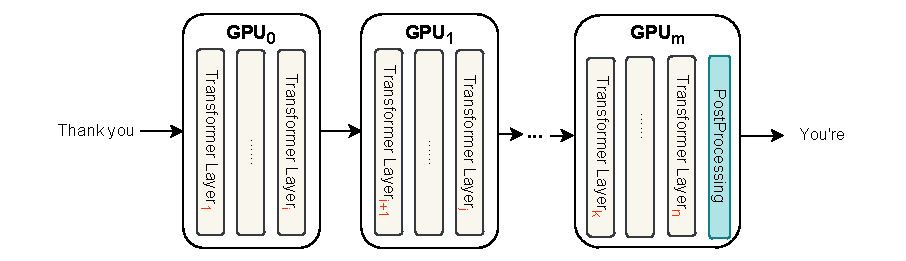
\includegraphics[width=3.3in]{figures/parallel_new_new_new.pdf}
% 		\caption{The pipelined parallelism}
% 		\label{Pipeline Parallelism}
% 	\end{minipage}
%     \label{LLM architecture}
% \end{figure}

% \begin{figure}[t] % 使用 [t] 尽量让图片置顶，符合论文习惯
%     \centering
%     % 第一张子图
%     \begin{subfigure}{\linewidth}
%         \centering
%         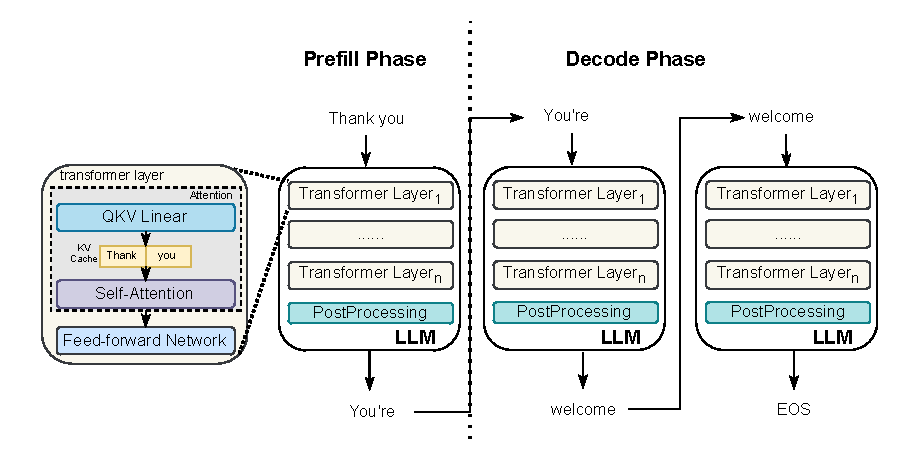
\includegraphics[width=3in]{figures/inference_phase_new_new_new.pdf}
%         \caption{The inference process of a transformer-based LLM model}
%         \label{fig:inferencephase}
%     \end{subfigure}
    
%     \vspace{1em} % 调节两张图之间的垂直间距，可以根据需要缩小或放大
    
%     % 第二张子图
%     \begin{subfigure}{\linewidth}
%         \centering
%         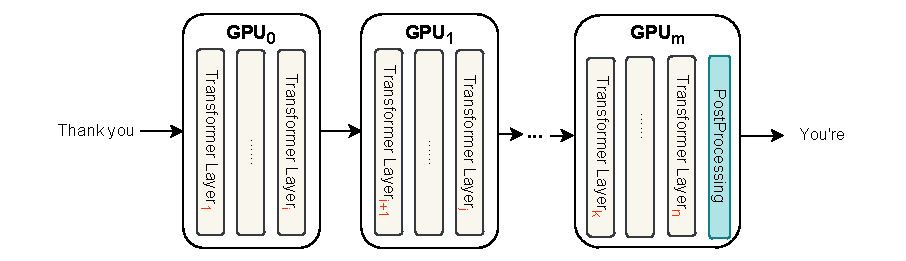
\includegraphics[width=3in]{figures/parallel_new_new_new.pdf}
%         \caption{The pipeline parallelism}
%         \label{Pipeline Parallelism}
%     \end{subfigure}
    
%     \caption{Overview of LLM inference and pipeline parallelism.} % 总标题
%     \label{fig:llm_architecture}
% \end{figure}

% \begin{figure}[t]
%     \centering
%     \begin{minipage}[t]{0.48\textwidth}
%         \centering
%         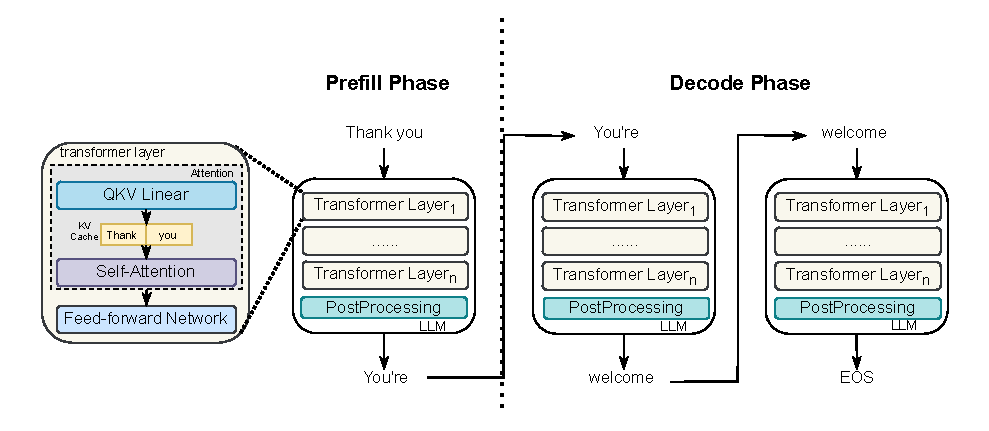
\includegraphics[width=\textwidth]{figures/inference_phase_new_new.pdf}
%         \caption{The inference process of a transformer-based LLM model}
%         \label{fig:inferencephase}
%     \end{minipage}
%     \hspace{0.02\textwidth}
%     \begin{minipage}[t]{0.48\textwidth}
%         \centering
%         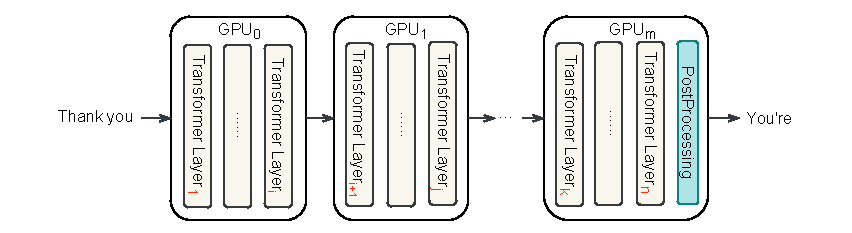
\includegraphics[width=\textwidth]{figures/parallel_new_new.pdf}
%         \caption{The pipelined parallelism}
%         \label{Pipeline Parallelism}
%     \end{minipage}
% \end{figure}

% \begin{figure}[t]
%     \centering
%     \begin{minipage}[t]{0.48\textwidth}
%         \centering
%         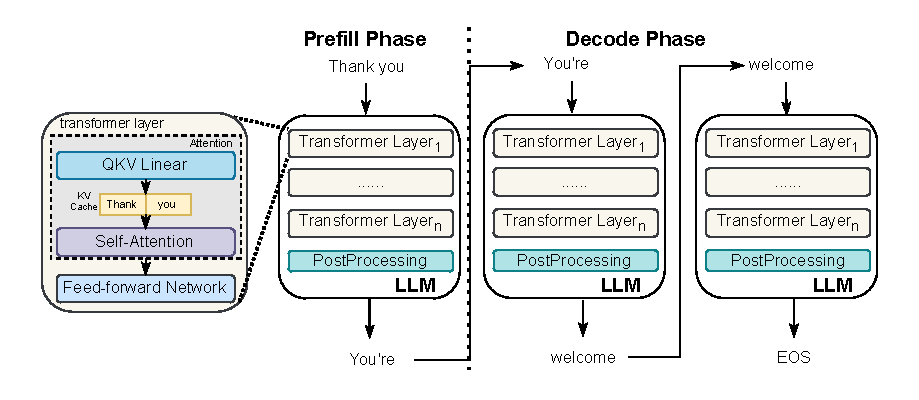
\includegraphics[width=\textwidth]{figures/inference_phase_new_new_new_new.pdf}
%         \caption{The inference process of a transformer-based LLM model}
%         \label{fig:inferencephase}
%     \end{minipage}
%     \hspace{0.02\textwidth}
%     \begin{minipage}[t]{0.48\textwidth}
%         \centering
%         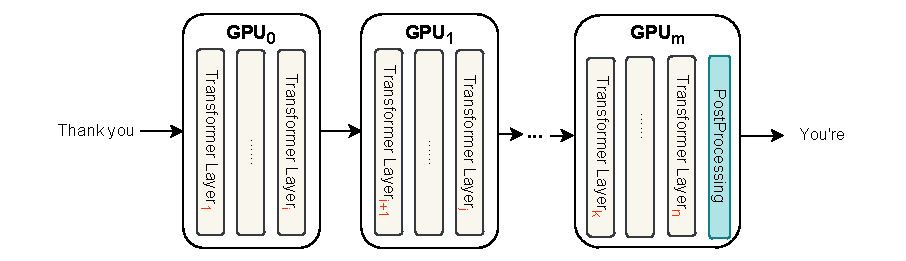
\includegraphics[width=\textwidth]{figures/parallel_new_new_new.pdf}
%         \caption{The pipelined parallelism}
%         \label{Pipeline Parallelism}
%     \end{minipage}
% \end{figure}

% \begin{figure}[t]
%     \centering
%     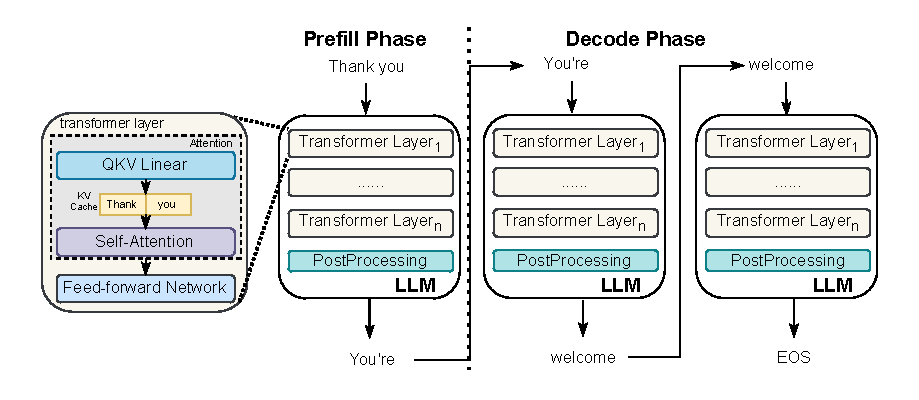
\includegraphics[width=0.48\textwidth, valign=m]{figures/inference_phase_new_new_new_new.pdf}
%     \hfill
%     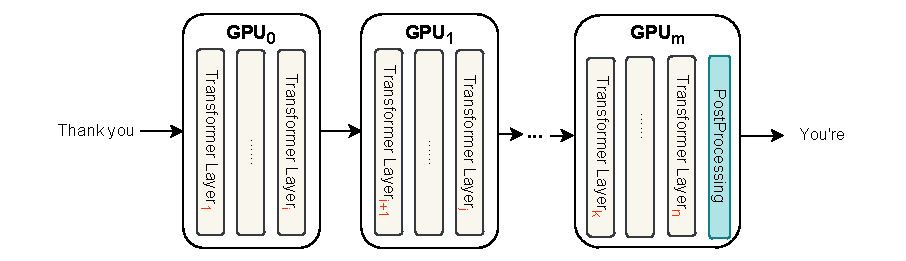
\includegraphics[width=0.48\textwidth, valign=m]{figures/parallel_new_new_new.pdf}
%     \begin{minipage}[t]{0.48\textwidth}
%         \caption{The inference process of a transformer-based LLM model.}
%         \label{fig:inferencephase}
%     \end{minipage}
%     \hfill
%     \begin{minipage}[t]{0.48\textwidth}
%         \caption{The pipelined parallelism mechanism.}
%         \label{Pipeline Parallelism}
%     \end{minipage}
% \end{figure}

% \begin{figure}[t]
%     \centering
%     % --- 第一行：图片部分（垂直居中对齐） ---
%     \begin{minipage}[c]{0.48\textwidth}
%         \centering
%         % 使用 \vfill 确保图片在 minipage 内部居中，或配合 \raisebox
%         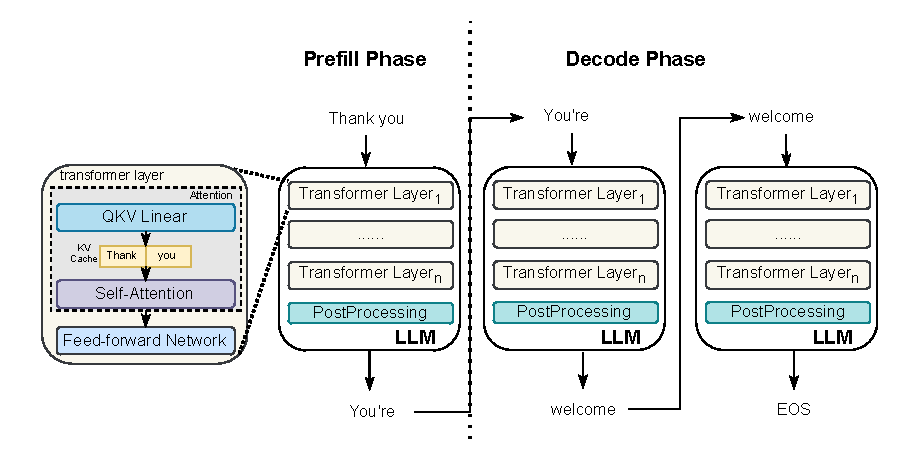
\includegraphics[width=\textwidth]{figures/inference_phase_new_new_new.pdf}
%     \end{minipage}
%     \hfill
%     \begin{minipage}[c]{0.48\textwidth}
%         \centering
%         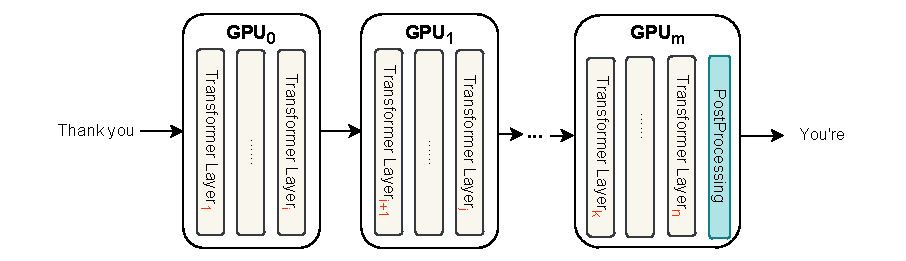
\includegraphics[width=\textwidth]{figures/parallel_new_new_new.pdf}
%     \end{minipage}

%     \vspace{5pt} % 调节图片与标题之间的间距

%     % --- 第二行：标题部分（顶端对齐，确保 Caption 对齐） ---
%     \begin{minipage}[t]{0.48\textwidth}
%         \caption{The inference process of a transformer-based LLM model}
%         \label{fig:inferencephase}
%     \end{minipage}
%     \hfill
%     \begin{minipage}[t]{0.48\textwidth}
%         \caption{The pipelined parallelism}
%         \label{Pipeline Parallelism}
%     \end{minipage}
% \end{figure}

% \begin{figure}[t]
%     \centering
%     % 创建一个两列表格，列宽各占约一半
%     \begin{tabular}{m{0.48\textwidth} m{0.48\textwidth}}
%         % --- 第一行：放图片 ---
%         \centering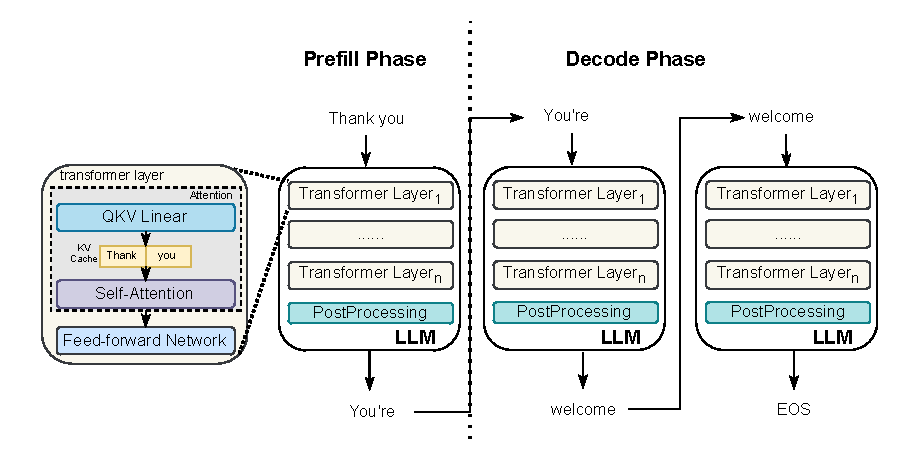
\includegraphics[width=0.45\textwidth]{figures/inference_phase_new_new_new.pdf} & 
%         \centering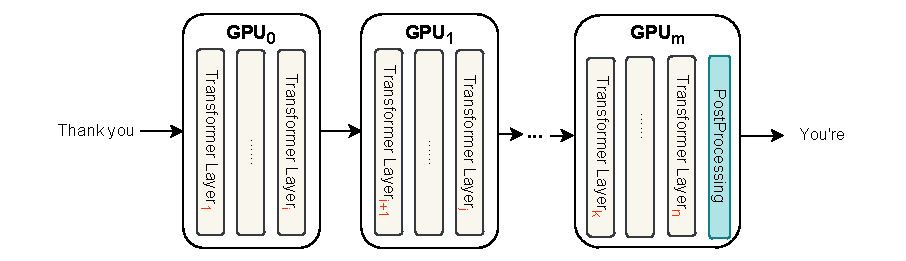
\includegraphics[width=0.45\textwidth]{figures/parallel_new_new_new.pdf} \\
        
%         % --- 第二行：放标题 ---
%         \begin{minipage}[t]{0.48\textwidth}
%             \caption{The inference process of a transformer-based LLM model}
%             \label{fig:inferencephase}
%         \end{minipage} & 
%         \begin{minipage}[t]{0.48\textwidth}
%             \caption{The pipelined parallelism}
%             \label{Pipeline Parallelism}
%         \end{minipage}
%     \end{tabular}
% \end{figure}

% \begin{figure}[t]
%     \centering
%     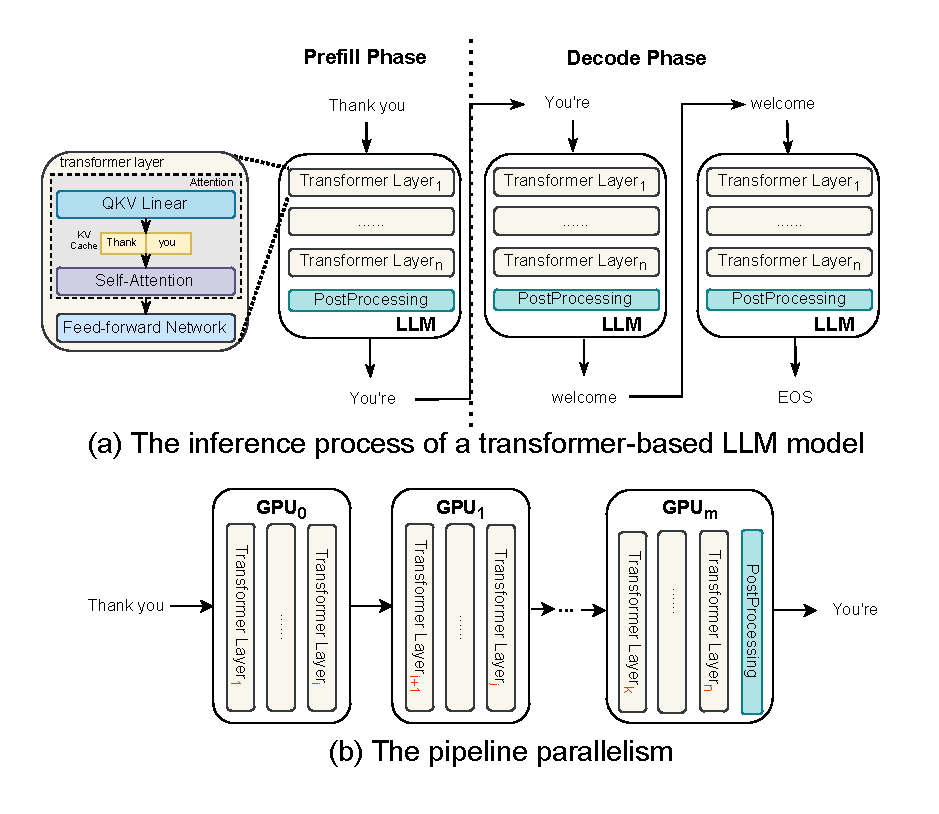
\includegraphics[width=0.7\linewidth]{figures/inference_phase_parallel.pdf}
%     \caption{Overview of LLM inference and pipeline parallelism.}
%     \label{fig:llm_architecture}
% \end{figure}

% Mainstream LLMs, such as ChatGPT \cite{achiam2023gpt}, Llama \cite{touvron2023llama}, and Gemini \cite{team2023gemini}, are built upon the transformer architecture, which consists of a sequence of identical transformer layers (referred to as "layers"). 
% Each layer contains two primary components: the \textit{Attention} and the \textit{Feed-Forward Network (FFN)}. 
% In the Attention, the input embeddings are projected into Query (Q), Key (K), and Value (V) vectors, and the interaction between Q and KV produces the attention outputs. 
% The FFN then further transforms these attention outputs through weight matrices to generate a hidden state as the input vector for the next layer. 
% As illustrated in Figure~\ref{fig:inferencephase}, an LLM processes $n$ layers sequentially within each iteration, producing a single token only after all layers are traversed. 
% This procedure repeats until an end-of-sequence (EOS) token is generated, with each iteration’s output concatenated with the prior context as input to the next iteration.

\bylyz{
An LLM consists of a sequence of Transformer layers (referred to simply as layers).
Each layer comprises an Attention module and a Feed-Forward Network (FFN). 
Within the Attention module, the input representation is first projected into Query ($Q$), Key ($K$), and Value ($V$) matrices. 
$Q$ then attends to $K$ and $V$ via scaled dot-product and Softmax operations to produce the output. 
The FFN subsequently takes the Attention output as input and performs two dense matrix multiplications to generate the input for the next layer. 
Finally, the hidden state output by the final layer undergoes an additional matrix multiplication and Softmax operation to sample from the vocabulary and generate the next token—a phase we denote as postprocessing.
}

% \bygpt{
% A decoder-only transformer LLM consists of a stack of transformer layers (hereafter referred to as layers). Each layer contains two main components: an attention module and a feed-forward network (FFN). The attention module first projects input hidden states into query (Q), key (K), and value (V) representations. Scaled dot products between Q and K are causally masked and normalized with softmax to obtain attention weights, which are applied to V to produce the attention output. The FFN then transforms the resulting hidden states through linear projections and nonlinear activations. Standard FFNs use two linear projections, whereas gated FFNs, such as those in Llama, use three. After the final layer, an output projection maps the hidden state to vocabulary logits. For sampling, softmax converts these logits into a probability distribution from which the next token is drawn. We refer to output projection and token selection together as postprocessing.
% }

% \bygemini{
% An LLM consists of a sequence of Transformer layers (referred to simply as layers). Each layer comprises an Attention module and a Feed-Forward Network (FFN). Within the Attention module, the input representation is first projected into Query ($Q$), Key ($K$), and Value ($V$) matrices. $Q$ then attends to $K$ and $V$ via scaled dot-product and Softmax operations to produce the output. The FFN subsequently takes the Attention output as input and performs two dense matrix multiplications to generate the input for the next layer. Finally, the hidden state output by the final layer undergoes an additional matrix multiplication and Softmax operation to sample from the vocabulary and generate the next token—a phase we denote as postprocessing.
% }

% Due to their distinct computational characteristics, the inference process can be divided into two phases:  
% \textbf{Prefill Phase:} The model processes the entire user request to generate the first token.  
% \textbf{Decode Phase:} The model then generates subsequent tokens in an auto-regressive manner, where each new token depends on all previously generated tokens.  
% Most LLM inference optimizations focus on the decode phase, as it accounts for the majority of inference time.

% During decoding, each newly generated Query must attend to all preceding Keys and Values to compute the attention output.
% We denote the number of preceding tokens as the \textit{sequence length}.
% Accordingly, the computational cost of the attention layer scales linearly with the \textit{sequence length}.
% To eliminate redundant recomputation of earlier KV pairs, LLMs employ a \textbf{KV-Cache}, which stores previously computed Keys and Values for direct reuse in subsequent iterations.
% In contrast, the FFN layer performs fixed-size matrix multiplications between the attention output and model parameters, making its computational cost independent of the sequence length.

% To improve computational efficiency and resource utilization, modern LLM inference engines adopt \textit{batching}, wherein multiple user requests are processed together as a single batch.
% Because LLMs contain an extremely large number of parameters, the cost of parameter loading is non-negligible.
% By aggregating embeddings from different requests into a matrix, batching allows computations to be executed as matrix multiplications instead of repeated vector operations and parameter loading, thereby enhancing efficiency.
% The number of requests processed together defines the \textit{batch size}.
% Consequently, the computational workload of a transformer layer increases proportionally with the batch size, in addition to a fixed but dominant parameter loading overhead.

\bylyz{
LLMs primarily operate in two phases: prefill and decode. 
During the prefill phase, the model processes the entire user request to generate the first output token. 
In the decode phase, it generates subsequent tokens iteratively using the newly generated token along with all preceding tokens, the count of which is referred to as the sequence length. 
This decoding loop repeats until an end-of-sequence (EOS) token is produced.
To avoid redundant Query-Key-Value (QKV) recalculations for previous tokens, LLMs employ a KV-Cache to store previously computed key and value states, loading them dynamically when needed.
Furthermore, to enhance computational efficiency, LLMs adopt batching, combining multiple user requests into a single batch to amortize the heavy overhead of loading model parameters. 
The total number of aggregated requests in a batch is defined as the batch size.
}

% \bygpt{
% LLM inference consists of two phases: prefill and decode. During prefill, the model processes the entire input prompt to produce the first output token. During decode, it generates subsequent tokens autoregressively, using the most recently generated token together with the preceding context. We use sequence length to denote the number of preceding context tokens, including prompt tokens and earlier generated tokens. Decoding continues until an end-of-sequence (EOS) token is generated or another stopping condition is met. To avoid recomputing the keys and values of previous tokens, the model stores them in a KV cache for reuse in subsequent iterations.
% To improve computational efficiency, inference engines group multiple requests into a batch, amortizing the cost of loading model parameters across these requests. The number of requests processed together in a batch is referred to as the batch size.
% }

% \bygemini{
% LLMs primarily operate in two phases: prefill and decode. During the prefill phase, the model processes the entire user request to generate the first output token. In the decode phase, it generates subsequent tokens iteratively using the newly generated token along with all preceding tokens, the count of which is referred to as the sequence length. This decoding loop repeats until an end-of-sequence (EOS) token is produced. To avoid redundant Query-Key-Value (QKV) recalculations for previous tokens, LLMs employ a KV-Cache to store previously computed key and value states, loading them dynamically when needed. Furthermore, to enhance computational efficiency, LLMs adopt batching, combining multiple user requests into a single batch to amortize the heavy overhead of loading model parameters. The total number of aggregated requests in a batch is defined as the batch size.
% }

\bylyz{
When an LLM becomes too large to fit on a single GPU, model parallelism distributes its parameters and computation across multiple GPUs.
Common strategies include tensor parallelism (TP), pipeline parallelism (PP), and expert parallelism (EP). 
TP partitions weight matrices within layers across GPUs and uses collective communication to combine intermediate results.
PP assigns groups of consecutive layers to different GPUs, which exchange activations at stage boundaries. 
Compared with TP, PP typically requires less frequent communication and can be more suitable for deployments with limited interconnect bandwidth, such as systems using PCIe.
EP targets mixture-of-experts (MoE) models, in which MoE layers contain multiple expert FFNs. 
It distributes these experts across GPUs and routes tokens to the selected experts.
Our work focuses on PP, while extensions involving other parallelism strategies are discussed in Section~\ref{sec:discussion}.
}

% \bygpt{
% When an LLM becomes too large to fit on a single GPU, model parallelism distributes its parameters and computation across multiple GPUs. Common strategies include tensor parallelism (TP), pipeline parallelism (PP), and expert parallelism (EP). TP partitions weight matrices within layers across GPUs and uses collective communication to combine intermediate results. PP assigns groups of consecutive layers to different GPUs, which exchange activations at stage boundaries. Compared with TP, PP typically requires less frequent communication and can be more suitable for deployments with limited interconnect bandwidth, such as systems using PCIe. EP targets mixture-of-experts (MoE) models, in which MoE layers contain multiple expert FFNs. It distributes these experts across GPUs and routes tokens to the selected experts. Our work focuses on PP, while extensions involving other parallelism strategies are discussed in Section~\ref{sec:discussion}.
% }

% \bygemini{
% As models grow larger and exceed the memory capacity of a single GPU, various parallel strategies have been proposed to shard parameters across multiple GPUs. The most commonly used strategies include Tensor Parallelism (TP), Pipeline Parallelism (PP), and Expert Parallelism (EP). Tensor Parallelism shards the weight matrices across GPUs, whereas Pipeline Parallelism partitions the model layer-by-layer. Pipeline Parallelism typically incurs lower communication overhead than Tensor Parallelism, making it better suited for systems with limited inter-GPU bandwidth, such as PCIe-interconnected nodes. Meanwhile, Expert Parallelism targets Mixture-of-Experts (MoE) models, where standard Feed-Forward Networks (FFNs) are replaced by multiple expert FFNs distributed across GPUs. Our work primarily focuses on the Pipeline Parallelism scenario, while other parallel strategies are discussed in Section \ref{sec:discussion}.
% }

%attention 和FFN都在干什么，矩阵乘法？里面有大量的参数需要加载，然后和输入的数据运算
%同时，还要和已经生成的数据运算
%因此一个layer的时间包括了模型加载，包括了blablabla，分别和什么相关。
%这样后面也可以说，batch其实是在提升这些数据的利用效率

% To improve computational efficiency and resource utilization, modern LLM inference engines adopt \textbf{batching}, where multiple user requests are processed simultaneously. 
% Specifically, embeddings from different requests are aggregated into a single matrix, allowing the computation to be executed as matrix multiplications rather than individual vector operations. 
% This design also enables model parameters, including those used for QKV projection and the FFN transformation, to be loaded once and reused across all requests in the batch, thereby reducing redundant memory accesses.
% The benefit of batching is particularly pronounced during the decode phase, where inference is typically dominated by parameter loading rather than arithmetic operations.
% \bygxl{!!!start the batch execution story here!!!}
%这里应该简单的提一句，batch的大小其实影响的是输入矩阵的大小，因此batch-size是每一个layer的推理时间的重要影响因素，就可以了。

% To improve computational efficiency and resource utilization, modern LLM inference engines adopt \textit{batching}, wherein multiple user requests are processed together as a single batch.
% Because LLMs contain an extremely large number of parameters, the cost of parameter loading is non-negligible.
% By aggregating embeddings from different requests into a matrix, batching allows computations to be executed as matrix multiplications instead of repeated vector operations and parameter loading, thereby enhancing efficiency.
% The number of requests processed together defines the \textit{batch size}.
% Consequently, the computational workload of a transformer layer increases proportionally with the batch size, in addition to a fixed but dominant parameter loading overhead.

% To enhance computational efficiency and resource utilization, LLMs typically batch multiple users' requests for inference by combining their embeddings into a matrix. 
% Matrix multiplications thus serve as the core operations and accounts for the majority of the inference time \cite{zhong2024distserve}. 
% The end-to-end execution time is also determined by the sizes of the input matrix and the parameter matrix, which in turn are dictated by the model size and the batch size.
% It is insensitive to the values stored in the matrices. 
% \bylyz{There}


% Due to differences in computational characteristics, the inference process is divided into two distinct phases:
% \textbf{Prefill Phase:} In this phase, the model processes the user’s request to generate the first token.
% \textbf{Decode Phase:} During this phase, the model generates subsequent tokens one-by-one in an auto-regressive manner. 
% The iterative nature of the model during decoding means that each new token is computed based on all previously generated tokens in the sequence. Specifically, the model relies on the Query, Key, and Value (QKV) matrices of the preceding tokens, leading to redundant regeneration of the Key and Value matrices for earlier tokens. 
% To mitigate this redundancy, LLMs store the previously computed Key and Value pairs in a \textbf{KV-Cache}. 
% As a result, the workload for generating each token is linearly proportional to the length of the sequence already generated. 
% This involves loading the KV pairs from the KV-Cache and computing the attention scores based on these stored values.





% % \notethis{say some conclusions about LLM inference}
%这里要说，有大量的计算，有大量的参数，因此GPU成了首选的计算设备
%还要说这个东西填不满一个GPU的算力，因此要做batch，我记得上一个论文里写了一段类似的话
%一个batch里面，session的多少，受到了GPU显存的限制
%别忘了在这一节的前半部分要强调这些tf block是相互独立的，结构都差不多，这样为后面引入流水线做文字上的铺垫

\subsection{Inevitable Bubbles in Pipeline-Based LLM Inference}
\label{sec:pipelinebubble}
%承担上文
%大模型的尺寸变大了，一个显卡放不下，需要多块卡共同存储，因此多卡也搞并行
%然后可以直接跳到，因为各个tf block是独立的，按块切开做流水是一个很直观的思路。注意就不要提其他的并行了，容易把主题搞散了

% LLM models impose intense memory pressure due to the large number of parameters in the transformer layers. 
% For instance, Llama2-70B consists of 80 layers, with each layer containing approximately 1 billion parameters.
% Additionally, the KV-Cache increases as the inference process progresses, consuming a substantial portion of GPU memory \cite{jin2023s}. 
% As a result, GPU memory capacity becomes a limiting factor for the number of layers and batches that can be deployed.

% Therefore, models are sharded across multiple GPUs in modern inference engines.
% This allows for larger batches, higher throughput, and more efficient inference.
% Pipeline parallelism (Figure~\ref{Pipeline Parallelism}) is a common strategy \cite{huang2019gpipe, rasley2020deepspeed}, where the \texttt{n} transformer layers are split into \texttt{m} stages, each on a separate GPU.
% Batches flow sequentially through the stages, and each GPU starts processing the next batch immediately after finishing the current one, boosting throughput.
% In the last stage, generated tokens are fed back to the first stage for the next iteration until an \texttt{EOS} token ends the process.

% Reducing pipeline bubbles is key to optimizing LLM inference.
\bylyz{Bubbles are commonly existed in the Pipeline Parallel and reducing these bubbles is key to optimizing LLM inference.}
Proposed solutions include stage alignment \cite{lin2024syncintellects,zheng2024response,jin2023s}, virtual pipeline stages \cite{narayanan2021efficient,jiang2024dynapipe}, and continuous batching \cite{yu2022orca}, the most widely used approach. 
In continuous batching, queued requests are grouped before inference, and new requests are added after each iteration when completed requests free enough GPU memory. 
This improves scheduling flexibility and GPU utilization \cite{achiam2023gpt,rasley2020deepspeed,devlin2018bert}.



\begin{figure}[t]
    \centering
    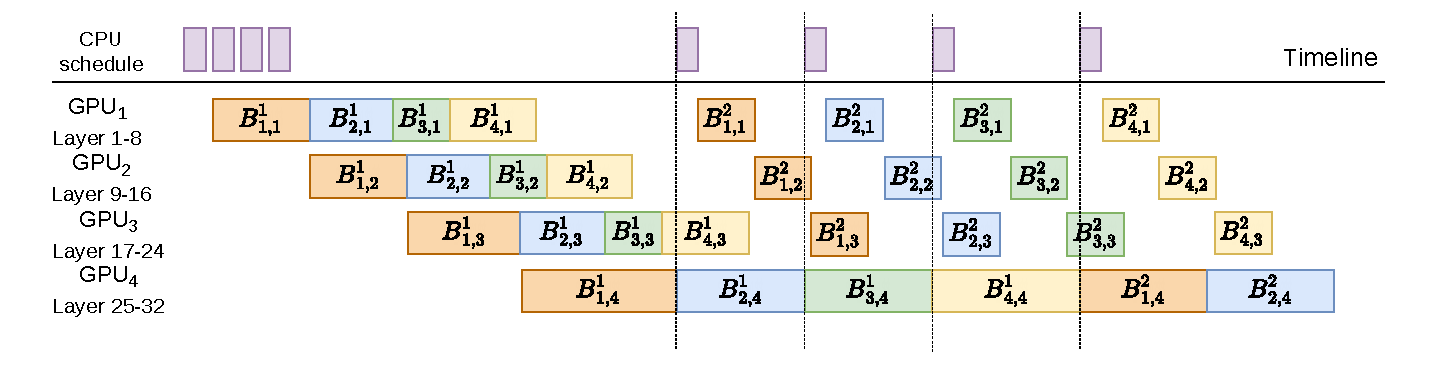
\includegraphics[width=0.9\linewidth]{figures/TACO_Rebuttal/workflow1_new.pdf}
    \caption{A schematic diagram of the timeline for a four-stage pipeline using continuous batching.}
    \label{workflow}
\end{figure}

Our observation shows that continuous batching cannot fully remove pipeline bubbles due to limited GPU memory.
Figure~\ref{workflow} illustrates a four-stage pipelined workflow utilizing continuous batching.
In this configuration, a 32-layer LLM is partitioned across four GPUs, with each GPU assigned a consecutive block of eight layers, forming one pipeline stage.
The purple segments indicate work performed by the CPU scheduling thread, which assembles batches by collecting requests from the waiting queue.
When a request reaches an \texttt{EOS} token, the scheduler returns the result to the user and releases its associated GPU memory.
Simultaneously, it schedules new requests to form the next batch.
Otherwise, it remains in the batch and proceeds to the next token generation iteration.
The brown, blue, green, and yellow segments represent inference threads on the GPUs, each responsible for executing a specific computational batch.
Specifically, $B_{i,j}^k$ denotes the $i$-th batch running on the $j$-th GPU (i.e., the $j$-th stage of the pipeline) during the $k$-th iteration, corresponding to generation of the $k$-th token.


\iffalse
\begin{table}
  \caption{Computational cost of various operations involved in generating a single token during the decoding phase, assuming a sequence length of 4096. "TL" denotes Transformer Layers, "P" denotes Projection and "S" denotes Sampling. $n$ denotes the number of transformer layers, and $N$ denotes the number of pipeline stages.}
  \label{tab:computation}
  \begin{tabular}{ccccc}
    \toprule
    \multirow{2}{*}{Model} & \multicolumn{3}{c}{Computation (GFLOPs)} & \multirow{2}{*}{Performance} \\
    \cmidrule{2-4}
     & TL & P+S & TL Per Stage \\
    % \midrule
    % Llama2-7B & \multirow{2}{*}{8.99 GFLOPs} & \multirow{2}{*}{0.26 GFLOPs} \\
    % $(n=32)$ & & \\
    \midrule
    Llama3-8B & \multirow{2}{*}{9.93} & \multirow{2}{*}{1.05} & \multirow{2}{*}{2.48 $(N=4)$} & \multirow{2}{*}{\Checkmark} \\
    $(n=32)$ & & & & \\
    \midrule
    Llama3-70B & \multirow{2}{*}{59.73} & \multirow{2}{*}{2.10} & 14.93 $(N=4)$ & \XSolidBrush \\
    $(n=80)$ & & & 7.47 $(N=8)$ & \Checkmark \\
    \bottomrule
  \end{tabular}
\end{table}
\fi

% memory constraint 导致了schedule的delay
At the start of an inference, the CPU scheduling thread and the inference thread on GPU$_1$ can run in parallel. 
While GPU$_1$ begins processing one batch, the CPU scheduler simultaneously constructs subsequent batches from the waiting queue to enable continuous batching inference. 
However, as the inference process advances, the available GPU memory capacity will be exhausted leaving insufficient memory to accommodate new batches.
In this case, the CPU must wait for the ongoing batch to complete before scheduling the next batch.
During this period, GPU$_1$ will be forced to stall and create a pipeline bubble.
This delay (or bubble) can ripple through the rest of the pipeline.  
As shown in Figure~\ref{workflow}, before the batch $B_{1,1}^2$ begins its execution, the CPU scheduling thread must wait for batch $B_{1,4}^1$ to complete its last stage on $\text{GPU}_{4}$ before it can assemble and schedule the next batch.
The pipeline bubbles are depicted as blank spaces between the colored fragments.
This memory constraint not only delays the current scheduling process but also impacts subsequent cycles, further propagating inefficiencies.

% schedule delay的时间取决于GPU3额外的计算量
% \bylyz{It is noteworthy that GPU3 has a longer execution time due to its additional workload that includes projection and token sampling.}
% Pipeline bubbles inherently arise from load imbalance across stages.
% In particular, the last stage incurs longer execution time because it performs additional \emph{postprocessing} operations.
% The \emph{postprocessing} stage consists of two steps:
% (1) \textit{Output projection}, a matrix multiplication where the weight matrix is determined by the vocabulary size of the model; and
% (2) \textit{Token sampling}, which applies a softmax to compute token probabilities followed by a sampling strategy (e.g., top-$k$) to select the next token.
% Due to the large vocabulary size, the computational overhead of \emph{postprocessing} is comparable to that of the transformer layers.
% For example, in the Llama3-8B model during the decode phase, a single transformer layer requires approximately 0.315 GFLOPs, whereas the \emph{postprocessing} stage requires about 1.05 GFLOPs, which is equivalent to the computation of 3.3 transformer layers.
\bylyz{
These pipeline bubbles inherently stem from workload imbalances across pipeline stages when memory capacity is insufficient to assemble a new batch. 
All stages except the last one process an equivalent number of Transformer layers with comparable computational overhead. 
In contrast, the last stage must perform additional postprocessing operations and accordingly incurs a longer execution time.
Due to the large vocabulary size, the computational overhead of postprocessing is comparable to that of multiple Transformer layers.
For instance, in the Llama3-8B model during the decoding phase, a single Transformer layer requires approximately 0.315 GFLOPs, whereas the postprocessing stage requires about 1.05 GFLOPs—an amount equivalent to the computation of 3.3 Transformer layers.
}

% \bygpt{
% Load imbalance across stages can contribute to pipeline bubbles. When transformer layers are evenly partitioned across identical GPUs, the stages have comparable computational workloads for layer execution. The last stage additionally performs \emph{postprocessing}, which can make it slower than the preceding stages. With a large vocabulary, output projection can require as much arithmetic work as several transformer layers. For example, for Llama3-8B during decoding with a sequence length of 4096, a theoretical count of the dominant matrix operations gives approximately 0.503 GFLOPs per transformer layer per token and 1.051 GFLOPs for output projection, counting a multiply-add as two FLOPs. Output projection alone therefore involves roughly 2.1 times the arithmetic work of a single transformer layer. The resulting execution-time increase also depends on memory traffic and implementation.
% }

% \bygemini{
% Pipeline bubbles inherently stem from workload imbalances across pipeline stages. All stages except the last one process an equivalent number of Transformer layers with comparable computational overhead. In contrast, the last stage must perform additional postprocessing operations and accordingly incurs a longer execution time. Due to the large vocabulary size, the computational overhead of postprocessing is comparable to that of multiple Transformer layers. For instance, in the Llama3-8B model during the decoding phase, a single Transformer layer requires approximately 0.315 GFLOPs, whereas the postprocessing stage requires about 1.05 GFLOPs—an amount equivalent to the computation of 3.3 Transformer layers.
% }

This imbalance cannot be resolved by redistributing model layers among the GPUs. 
The pipeline is divided based on the transformer layers in the LLM model, where each layer entails a similar computational workload and requires comparable GPU memory for model parameters and KV cache, as discussed in Section~\ref{sec:llmandtransformer}. 
Due to the limited GPU memory capacity, each GPU must handle an equal number of transformer layers to maintain a balanced pipeline infrastructure when using identical GPUs.
Re-balancing the pipeline by shifting some transformer layers from the last GPU to the preceding ones is not feasible.
% Furthermore, even if some layers from the last stage were migrated to earlier stages, it is still hard to fully eliminate the imbalance due to the coarse granularity of layer-level partitioning.
Furthermore, even if some layers from the last stage were migrated to earlier stages, it remains difficult to eliminate imbalance due to the coarse granularity of layer-level partitioning


The imbalance persists across different model scales.
Larger models typically require more GPUs to accommodate their vast number of parameters, which increases the number of pipeline stages.
As a result, each stage contains fewer transformer layers, while the additional workload of the last stage remains constant.
This structural asymmetry ensures that the imbalance does not disappear.
For example, the Llama3-8B model has 32 transformer layers and is commonly deployed on 4 GPUs, resulting in approximately 8 layers per stage.
In contrast, the Llama3-70B model contains 80 layers and is often deployed on 8 GPUs, yielding about 10 layers per stage.
Although the number of layers per stage grows in larger models, the extra \emph{postprocessing} computation is still confined to the last stage.


To quantify the imbalance, we conduct empirical measurements.
We deploy the Llama3-8B model on four NVIDIA RTX 3090 GPUs and the Llama3-70B model on eight NVIDIA A100 GPUs.
The ShareGPT dataset~\cite{chiang2023vicuna} is used as the inference workload.
We record the execution time of each pipeline stage, with results shown in Figure~\ref{fig:lifecyclepower}.
For clarity, we report the average execution time across all stages except the last one given these stages contain an identical number of layers (marked as \emph{Other Stage}), while the execution time of the last stage is reported separately as \emph{Last Stage}.
We also measure the duration of pipeline bubbles, defined as GPU idle periods between batches, and denote them as \emph{IDLE}.
This demonstrates that the last stage takes significantly longer to execute than the other stages.
Furthermore, the idle durations are notably brief (\hcwplaceholder{XXX} ms for Llama3-8B and \hcwplaceholder{XXX} ms for Llama3-70B), rendering dynamic adjustment techniques ineffective for reducing these bubbles.
%In Llama3-8B, its execution time exceeds that of the preceding stages by 6.6\% on average, and by 3.2\% in Llama3-70B.
%This prolonged last stage, combined with pipeline bubbles, results in substantial GPU idle time during inference. 
%In Llama3-70B, idle time can account for up to 60.4\% of total inference time, whereas in Llama3-8B, it can reach as high as 33.1\%.

% It is evident that GPU idle time, caused by pipeline bubbles, occupies a significant portion of the total inference time.
% In Llama3-70B, the idle time can account for up to 33.09\%, while in Llama3-8B, it can reach as high as 60.36\%.


% \begin{figure}[t]
%     \centering
%     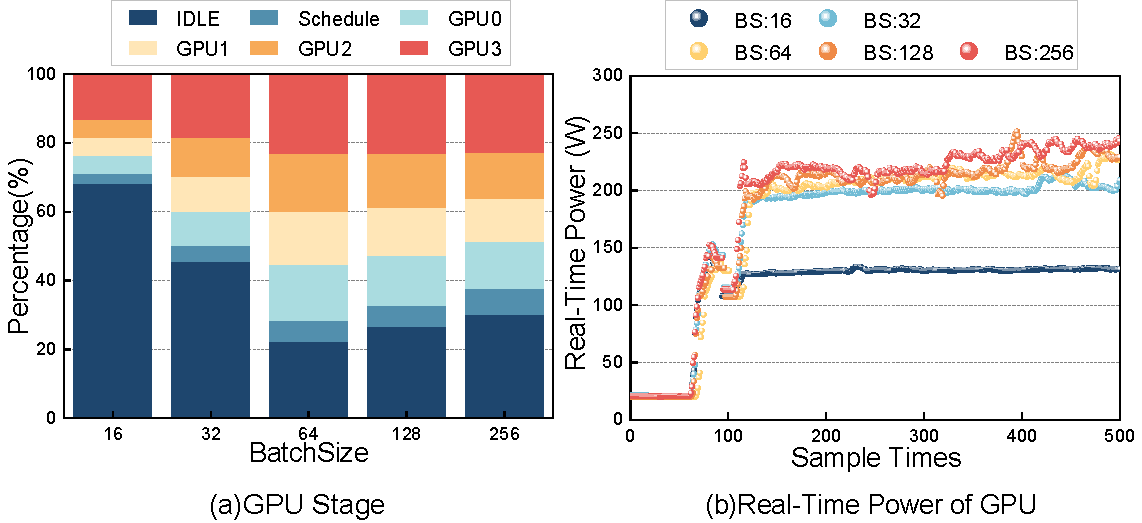
\includegraphics[width=1\linewidth]{figures/lifecycle_power_nq_new.pdf  }
%     \caption{(a) The distribution of the execution time in different stages running on four GPUs. (b) Real-time power usage in a parallel inference with different batch sizes.}
%     \label{fig:lifecyclepower}
% \end{figure}

% \begin{figure}[t]
%     \centering
%     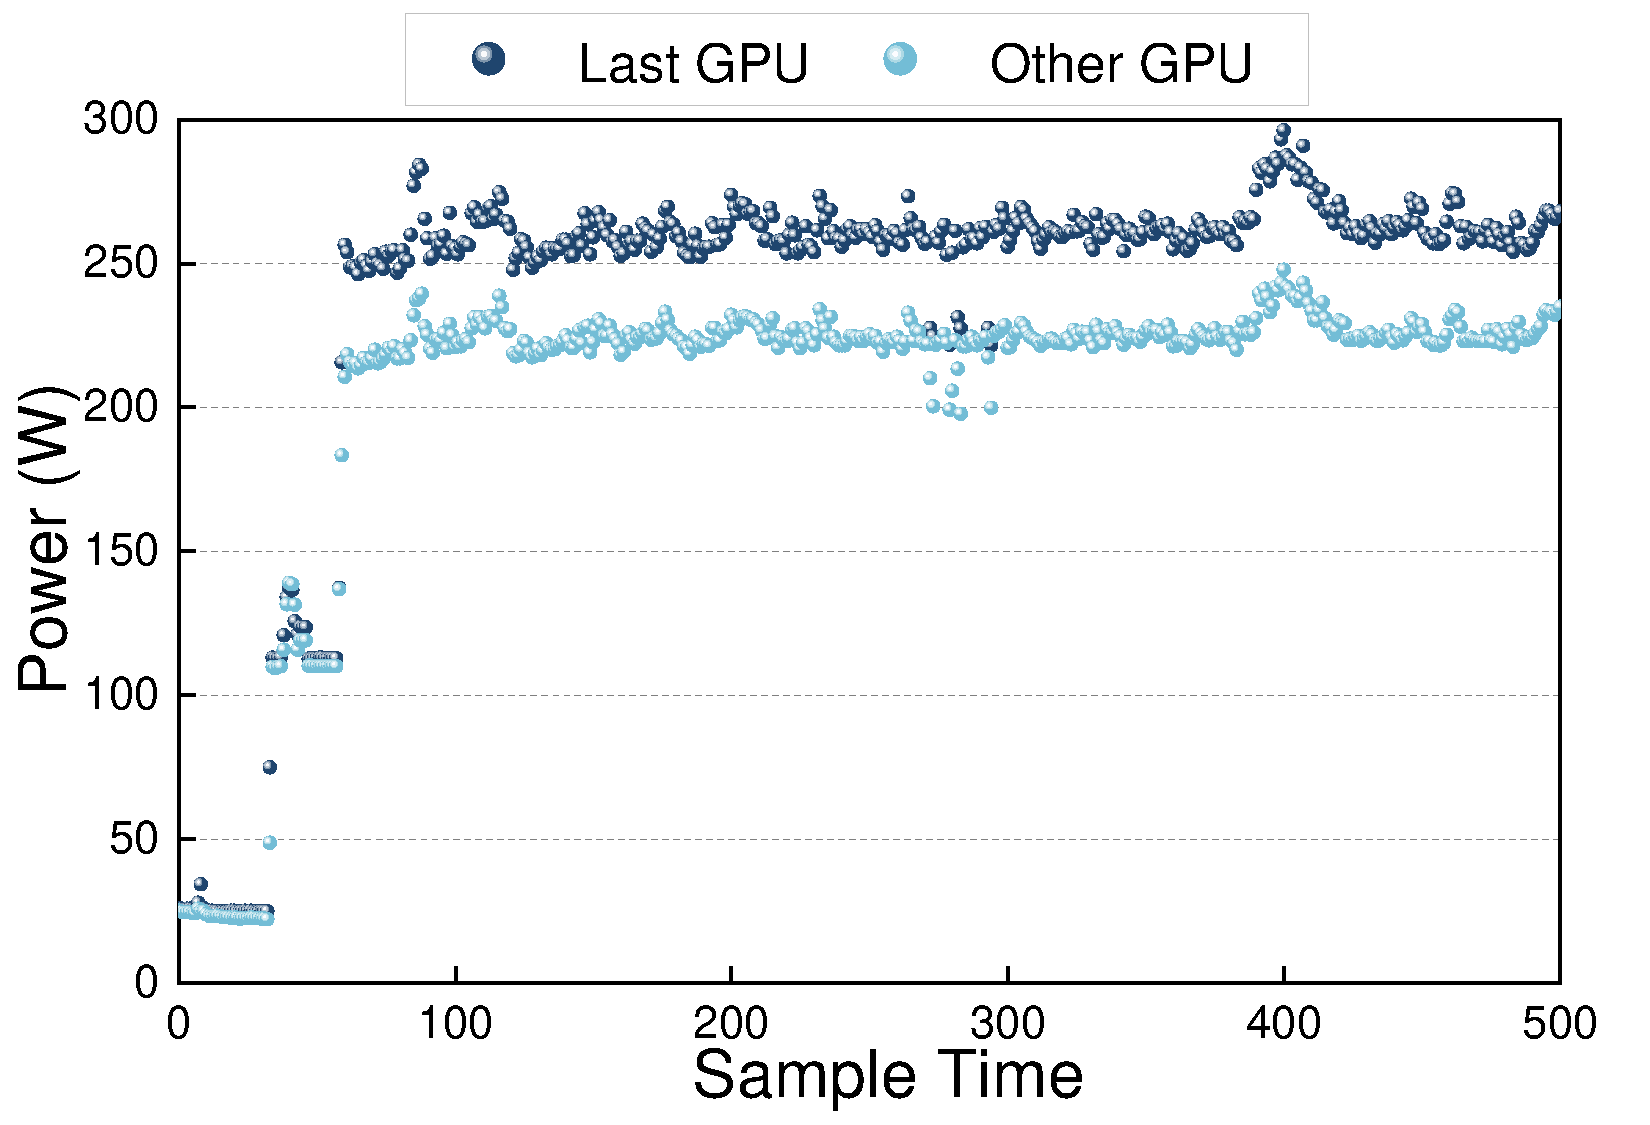
\includegraphics[width=0.9\linewidth]{figures/real_time_power.pdf}
%     \caption{Real-time power usage using the Llama3-8B model with four pipeline stages on RTX 3090 GPUs.}
%     \label{power-runtime}
% \end{figure}

% Figure 5
% \begin{figure}[t]
%     \centering
%     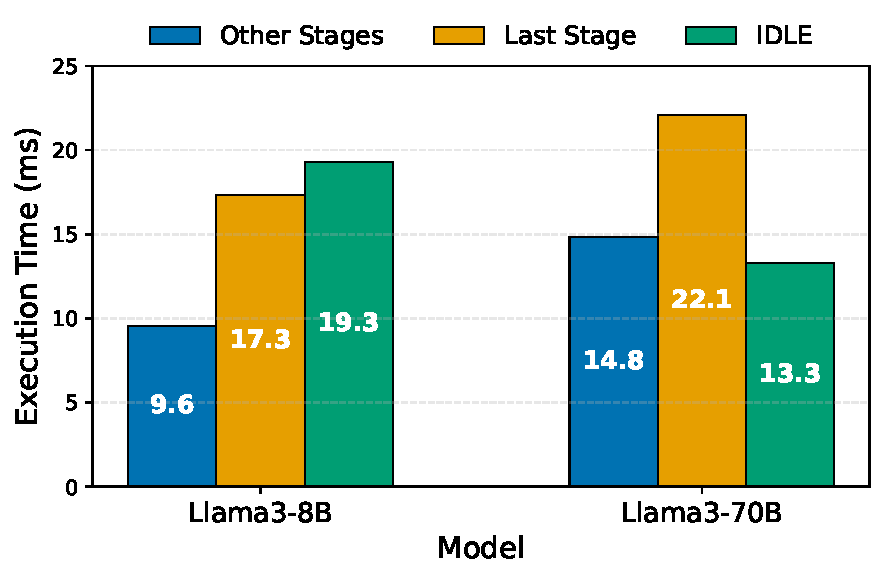
\includegraphics[width=0.9\linewidth]{figures/lifecycle_power_nq_new_new_new_new_new_new_new_new.pdf}
%     % \caption{(a) The distribution of the execution time in different stages. (b) Real-time power usage in a parallel inference for Llama3-8B.}
%     \caption{Execution time across pipeline stages for Llama3-8B and Llama3-70B.}
%     \label{fig:lifecyclepower}
% \end{figure}

% Figure 6
% \begin{figure}[t]
%     \centering
%     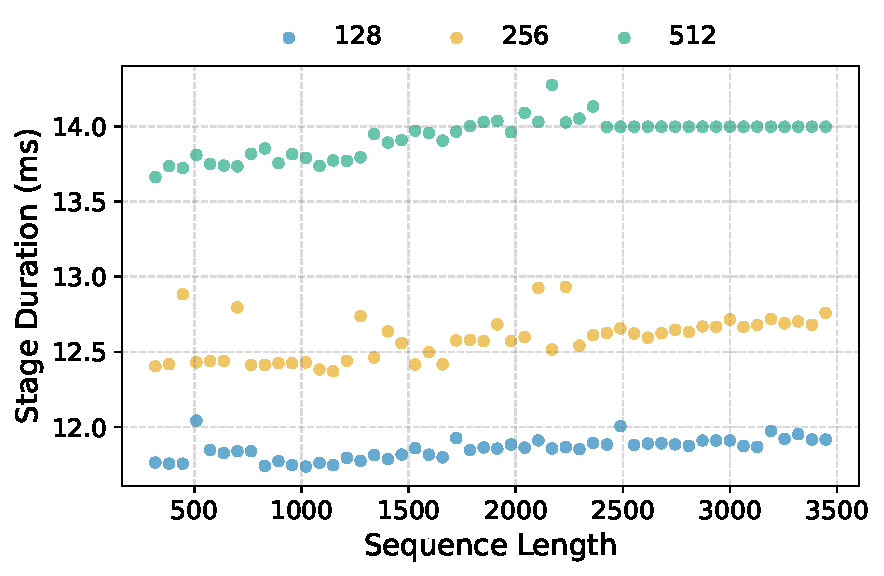
\includegraphics[width=0.9\linewidth]{figures/duration_seqlen_new_new.pdf}
%     \caption{Stage duration of Llama3-70B across different sequence lengths under batch sizes of 128, 256, and 512. Each color corresponds to a distinct batch size configuration.}
%     \label{fig:duration_seqlen}
% \end{figure}

% Figure 5 And 6
\begin{figure}[t]
    \centering
    \begin{minipage}[t]{0.48\textwidth}
        \centering
        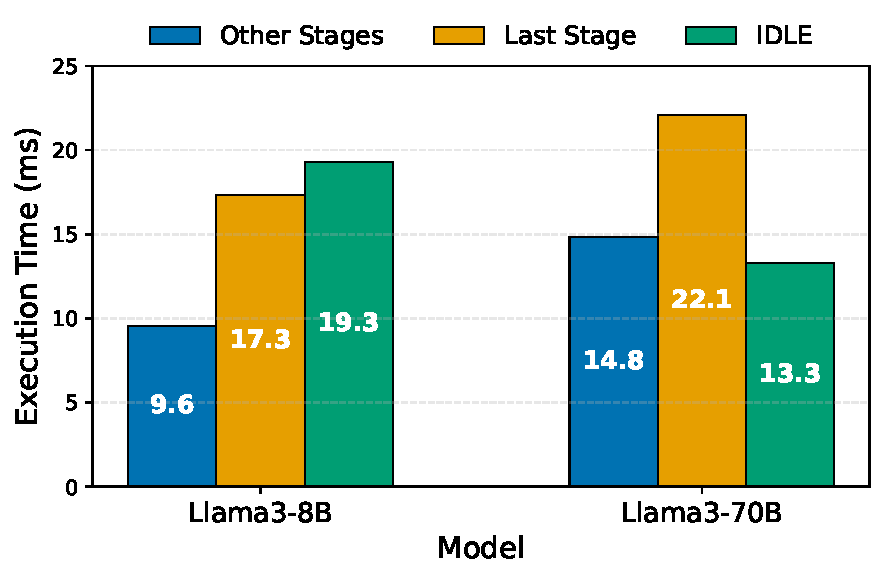
\includegraphics[width=\textwidth]{figures/lifecycle_power_nq_new_new_new_new_new_new_new_new.pdf}
        \caption{\lyzcheck{Execution time across pipeline stages for Llama3-8B and Llama3-70B.(x is model(Llama3-8B, Llama3-70B, \hcwplaceholder{XX}), y is Stage Execution Time. Try to make that other stage + idle = last stage)}}
        \label{fig:lifecyclepower}
    \end{minipage}
    \hspace{0.02\textwidth}
    \begin{minipage}[t]{0.48\textwidth}
        \centering
        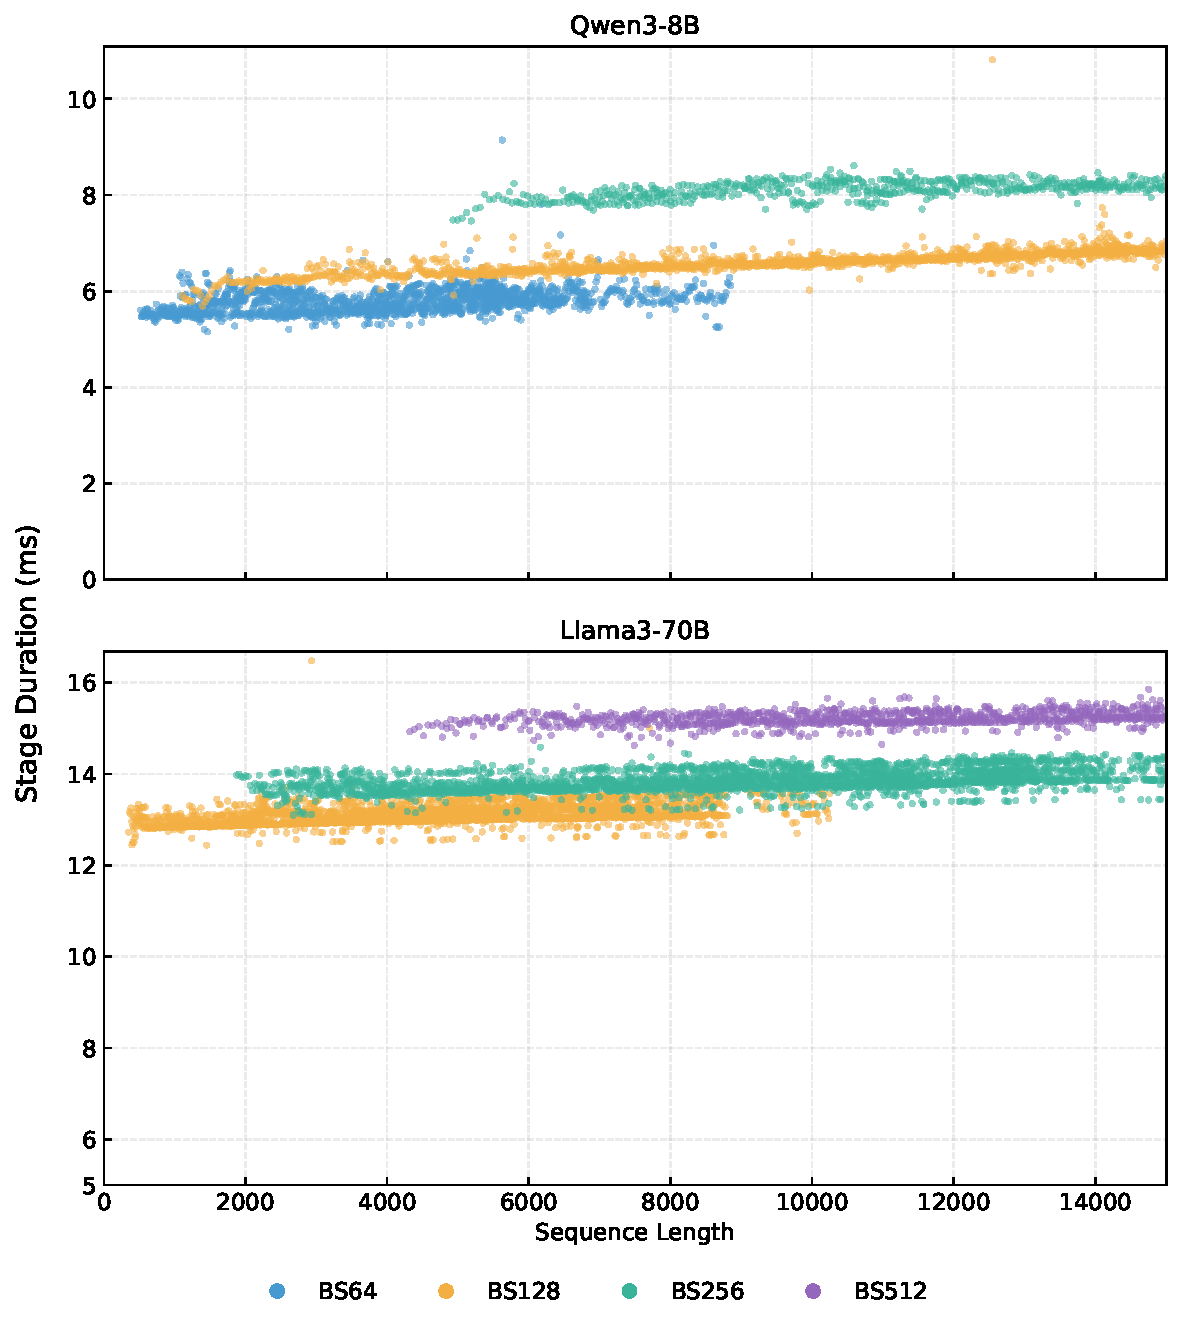
\includegraphics[width=\textwidth]{figures/hcw_final_figures/Fig4_auto_context_main_range_20261017.pdf}
        \caption{\byhcw{Middle-stage decode time versus aggregate batch context length on ShareGPT. Llama3-8B (Sarathi) is above Llama3-70B (SGLang); colors denote batch sizes. Two clipped Llama3-8B timing spikes are marked by triangles.}}
        \label{fig:duration_seqlen}
    \end{minipage}
\end{figure}

%However, the idle state of GPUs does not contribute to energy saving. 
%This leads to unnecessary power consumption, which adversely affects the overall power and energy efficiency of the system.


% \subsection{Execution Time of Stages}
\subsection{Stable Execution Time of Stage}
\label{sec:stableexecutiontime}
% The execution of a batch is stable

% \bygxl{See the comments.}
%每一个推理的任务是由Transformer+PostProcessing构成的
%Transformer的Attention部分和sequence length相关
%同时，各种优化技术【加参考文献】都在优化这一部分，减少sequence length对它的影响
%FFN只和模型相关
%因此，一个request的一个stage的时间，基本上是稳定的
%上例子，说明对于batch固定的时候，sequence length在变化，但是stage execution time是不变的
%另起一段
%同理，按照2.2节的分析，post processing也是不变的
%再起一段
%batch的大小，也就是一个stage中request的数量，会导致stage的时间scale up linearly
%分析原因，因为一个request是一个tensor，一个batch是把tensor合并成了matrics，batchsize就是matricx的行数
%However, 对于不同的batchsize, Ts/Tf是一个稳定的值，以及Ts(p1)/Ts(p0)是一个稳定的值（主要是表达这些东西与batchsize无关），看看
%结论段：虽然每一个调度的Batchsize不同，但因为比例相同，因此给了我们利用power cap调整stage并对齐执行时间的机会

% However, batchsize 是实时变化的by the scheduler to select the input prompts by user which is random.
% 这个random的prompts导致了batchsize符合正态分布，从而导致

According to the analysis in Section~\ref{sec:llmandtransformer}, several factors may influence the execution time of each stage, including \textit{sequence length} and \textit{batch size}.
However, our observations show that \textit{sequence length} has only a limited impact on stage execution time, particularly during the decode phase, which dominates the overall inference cost.




While the computation overhead of the Attention scales linearly with \textit{sequence length}, recent GPU kernels such as FlashDecoding++~\cite{hong2023flashdecoding++} and FlashInfer~\cite{ye2025flashinfer} substantially weaken this dependency by reorganizing memory access (e.g., double-buffered tiling) and introducing block-sparse KV storage.
Moreover, the FFN consistently dominates layer computation—accounting for roughly \hcwplaceholder{XX}--\hcwplaceholder{XX}\% of decode time compared with \hcwplaceholder{XX}--\hcwplaceholder{XX}\% for Attention~\cite{cheng2025ecco}—and its matrix multiplications are independent of sequence length.
Together, the dominance of sequence-independent FFN compute and the efficiency of optimized attention kernels ensure that stage execution time exhibits minimal sensitivity to sequence length in practice.

\byhcw{Using ShareGPT at Auto GPU frequency, we measure the mean middle-stage decode time for Llama3-8B on four RTX 3090 GPUs with Sarathi and Llama3-70B on eight A100 GPUs with SGLang. The horizontal axis in Figure~\ref{fig:duration_seqlen} is the sum of request context lengths in a pure-decode batch. At BS256, the median stage time increases by only 0.38 ms for Llama3-8B and 0.27 ms for Llama3-70B when comparing aggregate context lengths of 5,000--6,000 and 14,000--15,000 tokens.}
Consistent with our findings, prior work reports only a 1.5\% increase when the sequence length grows from 1000 to 4000 tokens~\cite{ye2025flashinfer}.
These results confirm that the impact of \textit{sequence length} on stage execution time is negligible.
Thus, the execution time of a stage can be regarded as stable under a predetermined \textit{batch size} configuration.

% Figure 6
% \begin{figure}[t]
%     \centering
%     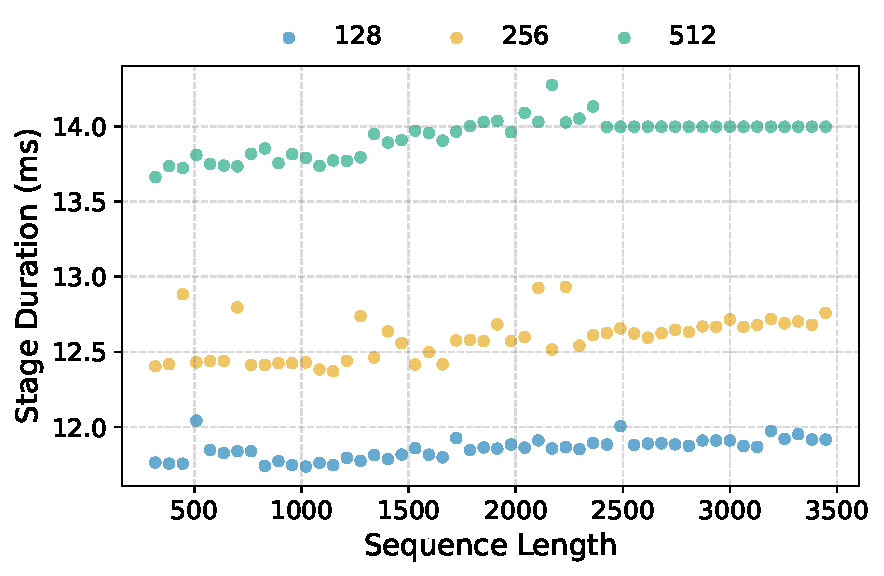
\includegraphics[width=0.9\linewidth]{figures/duration_seqlen_new_new.pdf}
%     \caption{Stage duration of Llama3-70B across different sequence lengths under batch sizes of 128, 256, and 512. Each color corresponds to a distinct batch size configuration.}
%     \label{fig:duration_seqlen}
% \end{figure}




\iffalse
\bylyz{
% Batch size is another factor that may influence stage execution time, as it determines the dimensions of matrices in both Attention and FFN computations. 
% In principle, larger batches lead to more FLOPs due to larger matrix multiplications. 
% Yet, during the decode phase, execution is typically dominated by parameter loading rather than arithmetic throughput. 
% Since model parameters are loaded once per batch regardless of its size, the per-batch execution time remains relatively stable across different batch sizes. 
Batch size is another factor that influences stage execution time. 
Larger batches increase the dimensions of the matrices in both Attention and FFN computations, leading to a theoretical increase in FLOPs. 
Yet during the decode phase, execution is predominantly memory-bound: parameter loading accounts for roughly 70--80\% of total time, while arithmetic operations contribute only 20--30\%~\cite{alizadeh2024llm, recasens2025mind}. 
Since model parameters are loaded once per batch and reused across requests, stage latency remains relatively stable across batch sizes despite the larger matrix operations. 
In practice, batch size cannot be increased arbitrarily because it is constrained by GPU memory capacity. 
For example, prior work reports that a single A100 GPU (40\,GB memory) can accommodate at most 200–300 concurrent sequences of length 1k when serving Llama-65B~\cite{alizadeh2024llm, kwon2023efficient}, and larger batch sizes quickly exceed memory limits. 
These constraints naturally bound the extent to which batch size affects runtime.  
}

\bylyz{
We empirically validate these observations through profiling experiments on eight A100 GPUs using the ShareGPT dataset. 
Here, we define the \textit{global batch size} as the total number of requests processed simultaneously across all running batches. 
Figure~\ref{fig:executiontime_dis} reports the distribution of per-stage latency under different global batch sizes. 
Although small variations exist, the overall latency remains within a narrow range (around 12--14 ms) across global batch sizes of 128, 256, and 512. 
This confirms that stage execution time is largely insensitive to both sequence length and batch size during the decode phase, reinforcing the assumption of runtime stability that underpins our analytical performance model in Section~\ref{sec:profiling}.
}

\begin{figure}[t]
    \centering
    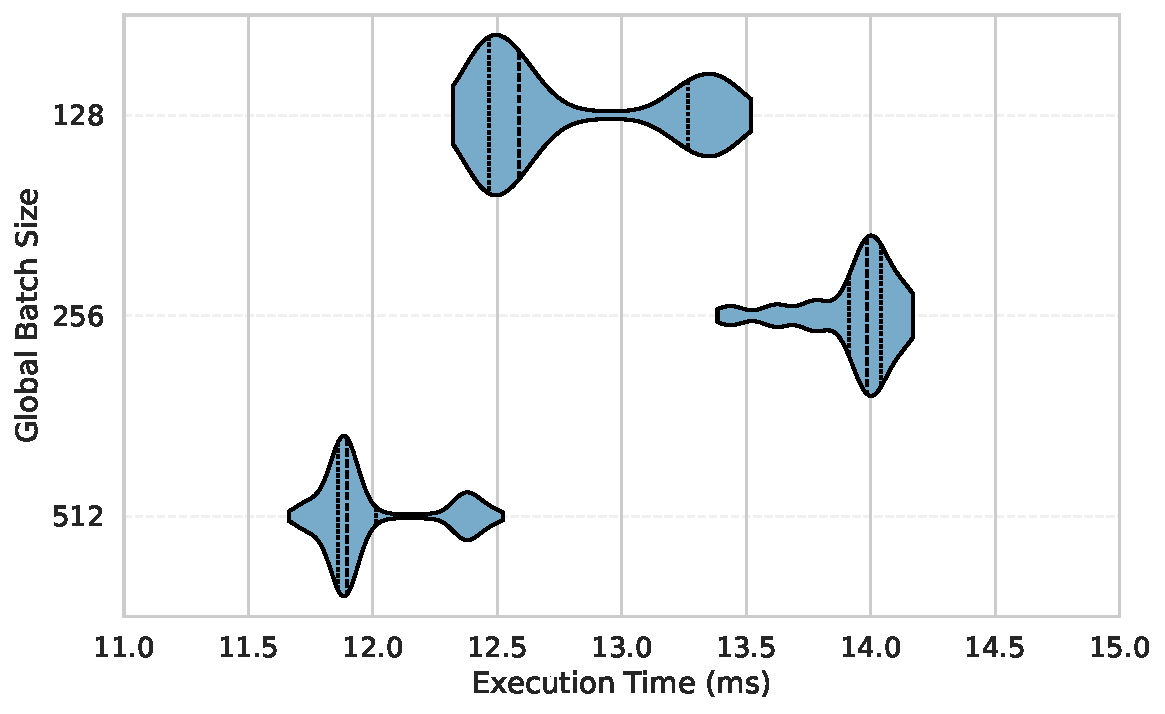
\includegraphics[width=0.9\linewidth]{figures/executiontime_dis.pdf}
    \caption{Distribution of batch execution times across Global Batch Sizes on the ShareGPT dataset using Llama3-70B on eight A100.}
    \label{fig:executiontime_dis}
\end{figure}

\fi



\subsection{GPU Frequency Management}


%1. 现在的GPU是支持电源管理的，但是这个东西根本帮不到我们，因为需要周期
%2. 电源管理的本质是主频的变化，也就是限制能耗会导致计算变慢
%3. 这两个东西之间是有数学关系的，可以是别人的相关研究，也可以是我们的实验
%4. 利用这个数学关系，可以指导我们填上这个气泡

% 现在的GPU可以通过负载自动调节性能状态

% Modern GPUs are equipped with advanced power management capabilities, enabling them to dynamically adjust power and energy consumption in response to varying computational load\cite{nvidia}. 
% Specifically, GPUs support multiple performance states (P-states), each characterized by different levels of power consumption and computational performance\cite{nvidia}. 
% These states allow parameters such as operating frequency and power usage to be tuned to match the demand of the workload, i.e., it will transition from a higher performance state (e.g., P0) to a lower one (e.g., P8).
% Such a dynamic adjustment can optimize the power consumption and achieve a balance between performance and energy efficiency.


\bylyz{
GPU core frequency is a configurable operating parameter that affects both energy efficiency and execution
time. Modern GPUs employ dynamic voltage and frequency scaling (DVFS) to adapt their operating conditions to
workload demands within power and thermal limits. However, these hardware-level policies do not necessarily exploit
the slack available between pipeline stages. Software-directed approaches can complement these policies by selecting
frequencies based on workload measurements or predictions.
However, these pipeline bubbles last only tens of milliseconds, making it challenging to monitor workload changes, select an appropriate frequency, and complete the frequency transition within such a short time window.
}

% \bygpt{
% GPU core frequency is a configurable operating parameter that affects both power consumption and execution time. Modern GPUs employ dynamic voltage and frequency scaling (DVFS) to adapt their operating conditions to workload demands within power and thermal limits. However, these hardware-level policies do not necessarily exploit the slack available between pipeline stages. Software-directed approaches can complement these policies by selecting frequencies based on workload measurements or predictions. For pipeline bubbles lasting only tens of milliseconds, workload monitoring, control decisions, and frequency transitions must be coordinated within short time windows. Their overheads depend on the GPU platform and control interface and can limit the benefits of adjusting frequencies in response to individual bubbles.
% }

% \bygemini{
% Frequency is a critical and configurable parameter in modern GPUs that directly influences both power consumption and computation latency. Although modern GPUs can dynamically adjust their frequency to reduce power based on workload fluctuations, relying solely on such automated mechanisms is typically insufficient because these adjustments lack adequate accuracy. Consequently, existing studies often focus on manually setting precise frequencies by capturing and predicting workload variations. However, these manual adjustments usually operate at a granularity of seconds or longer, whereas pipeline bubbles frequently last for only tens of milliseconds. Such brief durations make it extremely challenging for GPUs to accurately detect workload shifts and apply appropriate frequency configurations in a timely manner.
% }


% Extensive research has been conducted on the dynamic power management of GPUs\cite{wang2021dynamic, bridges2016understanding, mercati2017multi, krzywaniak2023dynamic}. 
% Generally, the adjustment process relies on the workload traces to regulate the power states at a granularity level of seconds or longer\cite{chen2023joss, singhania2024methodology}. 
% However, in an LLM inference, pipeline bubbles often last only tens of milliseconds. 
% Such short periods make it challenging for GPUs to accurately detect workload changes and adjust their power states accordingly.
% \bygxl{Not sure if correct. Change it when necessary.}



%The fine-grained time scale further complicates manual adjustments to the GPU power state in response to rapidly changing demands. As a result, existing solutions are inadequat e for achieving dynamic power adjustments during runtime to accommodate fluctuating computational needs.Therefore, it is difficult for existing technical methods to achieve dynamic power adjustment at runtime to adapt to changing computing tasks. 


%Although the GPU's automatic power management does not effectively address the energy consumption issues caused by pipeline bubbles, it has led us to an important insight. We identified that the core of power management lies in adjusting the GPU's power, controlling energy consumption by modifying power levels, and adapting computational capacity to meet varying load demands. Through experimental analysis, this paper reveals a mathematical relationship between power and program performance. This finding offers a new approach: by adjusting the GPU's power, we can manipulate its computation time, effectively filling pipeline bubbles and optimizing overall energy efficiency.